\chapter{Architectural Details of ``Sapphire Rapids'' Processors}
The Sapphire Rapids family of Server Processors is the successor to the ``Ice Lake'' architecture.
It is the first in Intels lineup of server processor to introduce a modular design containing four tiles in a 2x2 grid interconnected with EMIB structures.
The two variants of this processor are the 4th Generation Intel Xeon Scalable Processor and Xeon CPU Max Series with four additional HBM blocks~\cite{Intel_2021_Hotchips}.
Each tile contains up to 15 Golden Cove cores with a shared L3 cache connected by a mesh, accelerators, two DDR5 memory busses, N PCIe Gen 5 and one UPI 2.0 link.
This structure enables the package to be used in a single memory domain or split into two or four sub-NUMA clusters~\cite{Intel_4th_gen_scalable}.
Unlike their predecessors, up to four cores in each tile row are connected to a shared FIVR~\cite{Intel_2022_ISSCC}.
This change adds an additional energy optimization domain for mixed-frequency workloads.

\todoms{In which direction is the row of the voltage regutlators?}
\todoms{Information about the four types of accelerators.}
\todoms{Information about the PCIe and DDR5}

\begin{figure}[]
    \centering
    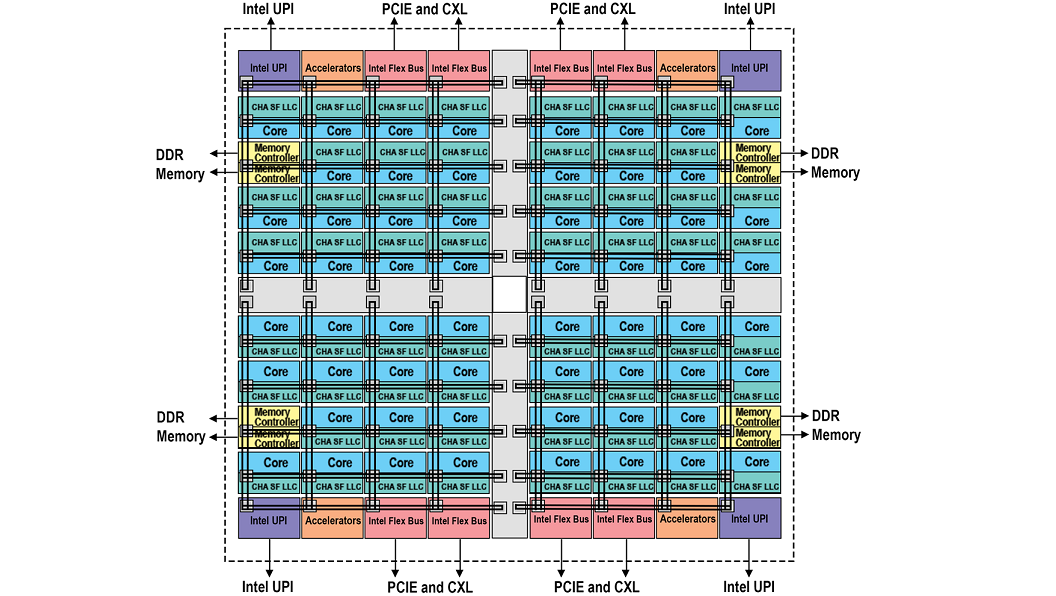
\includegraphics[width=\columnwidth]{fig/spr-uma.png}
    \caption{Block diagram of the 4th Generation Intel Xeon Scalable Processor from~\cite{Intel_4th_gen_scalable}.
Two mirrored tiles are arranged in a 2x2 grid, which are interconnected with EMIB structures to continue the mesh across the die boundaries.~\cite{Intel_2022_ISSCC}}
\end{figure}

\todoms{Show test system detail table.}

\todoms{Show the physical structure of the cores. Measure the memory core to core latency and plot it.
create a diagram with the active and unactive cores numbered in the plot.
Where is the PMU?}

\section{Golden Cove Core Microarchitecture}

\begin{figure}[]
    \centering
    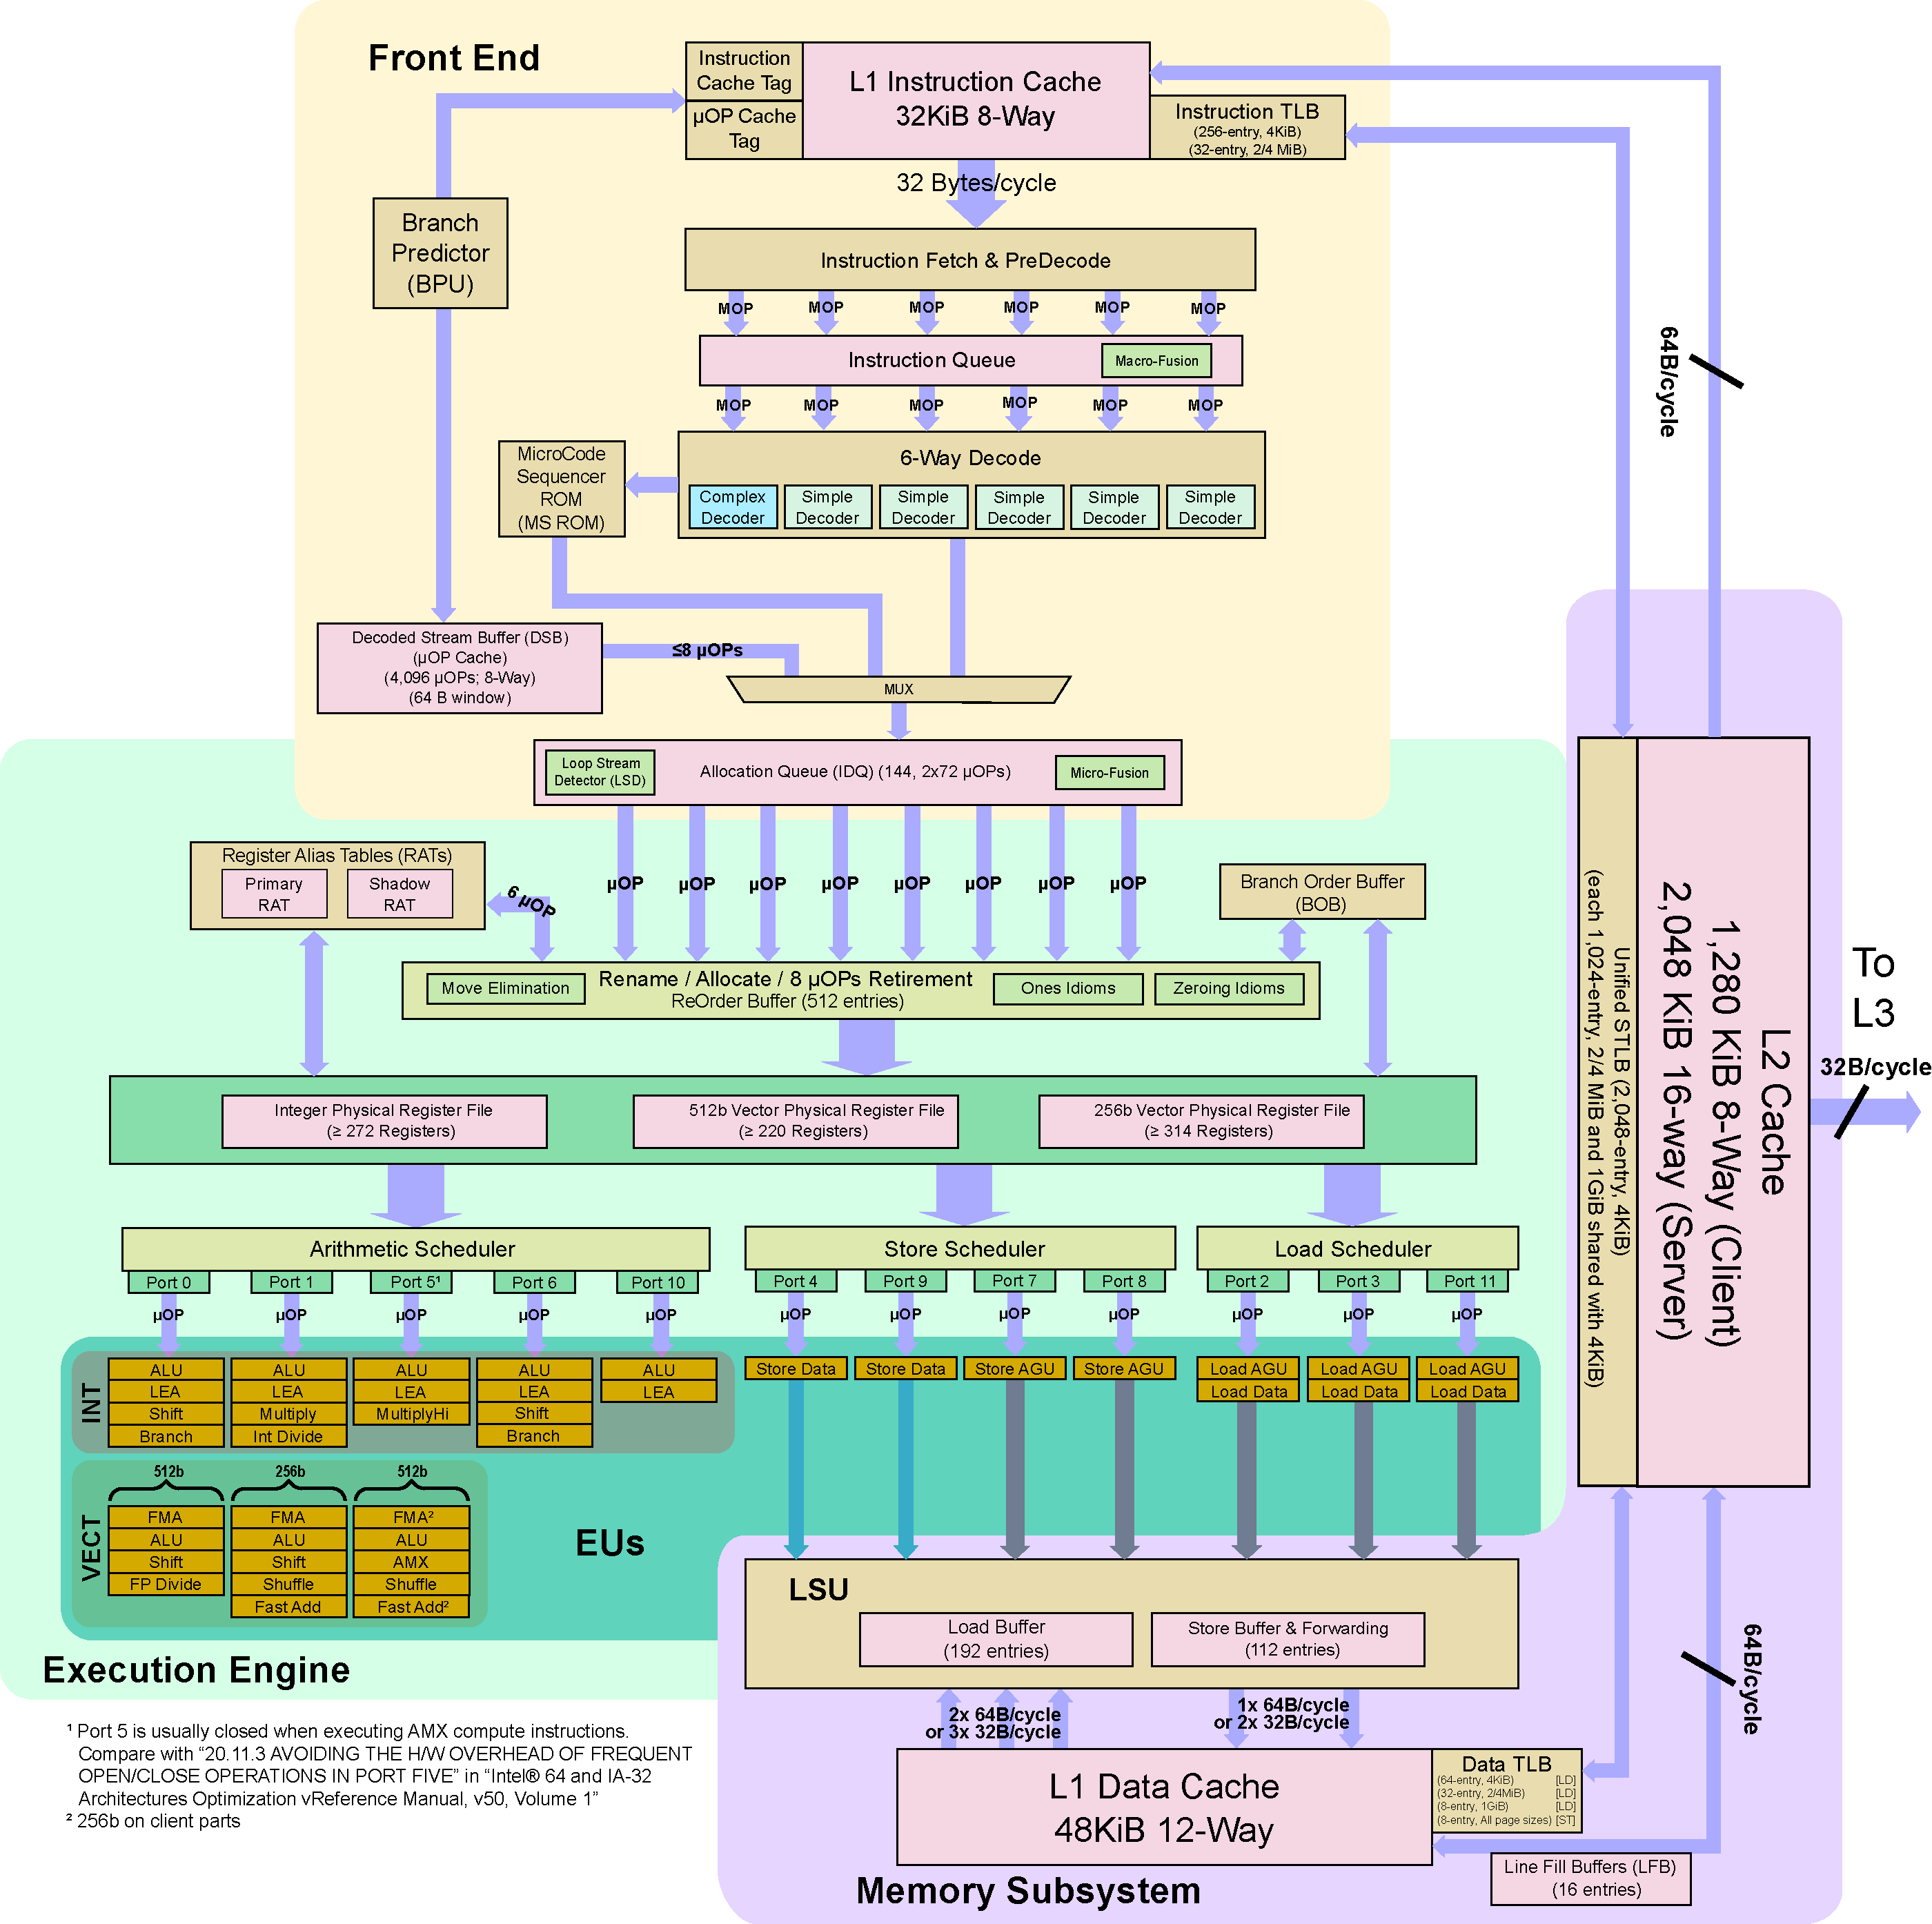
\includegraphics[width=\columnwidth]{fig/GoldenCoveCore.pdf}
    \caption{Block diagram of the Golden Cove Core.}
    \todoms{Measurements for the schedulers. How did the frontend change? Details of port 5 closing.}
\end{figure}